\documentclass[A4,10pt,greek]{book}
\usepackage{xltxtra}
\usepackage{xgreek}
\usepackage[a4paper, inner=1.5cm, outer=3cm, top=2cm, bottom=3cm, bindingoffset=1cm]{geometry}
\setmainfont[Mapping=tex-text]{GFS Didot}
\usepackage{amsfonts}

\title{Εφαρμογή Μισθοδοσίας M13 δοκιμή}
\author{Λάζαρος Θεόδωρος- Παναγιώτου Σπύρος}

\begin{document}
\maketitle

\tableofcontents

\frontmatter
\chapter{Πρόλογος}
Η δημιουργία πλήρους προγράμματος για την διαχείρηση της Ελληνικής μισθοδοσίας, αποτελεί πρόκληση διότι:
\begin{enumerate}
\item Υπάρχει μεγάλος αριθμός παραμέτρων και εξαιρέσεων που θα πρέπει να ληφθούν υπ'όψιν.
\item Υπάρχει αλληλεπίδραση μεταξύ των παραμέτρων.
\item Οι Νόμοι του Κράτους σχετικά με τα θέματα της μισθοδοσίας αλλάζουν συχνά. 
\item Υπάρχει πληθώρα επικουρικών ταμείων , το καθένα από αυτά με διαφορετικούς τρόπους υπολογισμού των κρατήσεων και με διαφορετικά δεδομένα για την επιχείρηση , την ειδικότητα και τον εργαζόμενο.
\item Επίσης δεν έχει δημιουργηθεί ακόμα standard xml για την επικοινωνία μεταξύ διαφόρων μισθολογικών προγραμμάτων, έτσι ώστε οι χρήστες να μην είναι κλειδωμένοι και περιορισμένοι στις τρέχουσες επιλογές τους.  

\end{enumerate}

Το βιβλίο αυτό φιλοδοξεί να γίνει ένας πλήρης οδηγός για τον προγραμματιστή και μιά ολοκληρωμένη βοήθεια για τον τελικό χρήστη. 

\mainmatter
\chapter{ Εργαλεία Προγραμματισμού}
Η εφαρμογή μισθοδοσίας είναι ανοικτό λογισμικό. Τα εργαλεία δημιουργίας της ανήκουν στο ανοικτό λογισμικό επίσης.

\section{ΕΛ/ΛΑΚ - GPL }
 To λογισμικό που χρησιμοποιώ είναι σε συντριπτικό ποσοστό ΕΛ/ΛΑΚ\footnote{Ελεύθερο Λογισμικό/Λογισμικό Ανοικτού Κώδικα} , προϊόν της ατομικής ή συλλογικής εργασίας προγραμματιστών που διαθέτουν δωρεάν την εργασία τους. Είμαι λάτρης της ιδέας του ΕΛ/ΛΑΚ , και σαν αποτέλεσμα το M13 είναι ανοικτό λογισμικό κάτω από την άδεια χρήσης GPL. 

\section{Απαραίτητα προγράμματα για εγκατάσταση}

\subsection{Python}
Γλώσσα προγραμματισμού Python\footnote{http://www.python.org}. Είναι δημιούργημα του Guido van Rossum και η ανάπτυξή του ξεκίνησε τον Δεκέμβριο του 1989 στην Ολλανδία. ΤΟ ΑΠΟΛΥΤΟ ΕΡΓΑΛΕΙΟ ΠΡΟΓΡΑΜΜΑΤΙΣΜΟΥ !!!

Για λόγους συμβατότητας με άλλα υποσυστήματα, εγκαθιστούμε την έκδοση 2.7 32bit.

\subsection{Δοκιμαστικό}
Μια δοκιμή για τη δύναμη του LAtex \footnote{Για το Σπύρο}.   

\subsection{sqlite}
Bάση δεδομένων  sqlite3\footnote{http://www.sqlite.org}.  Είναι μια πλήρης σχεσιακή βάση δεδομένων που τρέχει στα περισσοτερα  λειτουργικά συστήματα, από mainfraimes έως τηλέφωνα. Είναι το βασικό εργαλείο αποθήκευσης δεδομένων για τις πλατφόρμες Android και apple OS  .Υπάρχει ενσωματωμένη σαν βιβλιοθήκη στον python. Τα αρχεία που αποθηκεύονται τα δεδομένα της εφαρμογής Μ13 είναι τύπου sqlite3. 

\subsection{PyQt}
Η διεπαφή γραφικών  PyQt\footnote{http://www.riverbankcomputing.co.uk}. Είναι μια βιβλιοθήκη της Python που στηρίζεται στην αντίστοιχη cross platform βιβλιοθήκη Qt . Πληρέστατη , ισχυρή και εύκολα επεκτάσιμη.

Εγκαθιστούμε την έκδοση που υποστηρίζει python 2.7

\subsection{Py2exe}
Βιβλιοθήκη της python\footnote{http://www.py2exe.org} για τη δημιουργία αυτοτελών, εκτελέσιμων από το περιβάλλον Windows, εφαρμογών.

\subsection{Inno Setup}
 Το inno setup\footnote{http://www.jrsoftware.org/isinfo.php} είναι εργαλείο που μετατρέπει το εκτελέσιμο που παράγει ο py2exe σε εφαρμογή εγκατάστασης για Windows.

\subsection{Eclipse}

\subsection {pydev}

\chapter{Τεχνικές προδιαγραφές}
\section{Γενικές γραμμές}
Η εφαρμογή υλοποιείται με βάση τις παρακάτω σχεδιαστικές επιλογές :
\begin{enumerate}
\item Έχει δοθεί έμφαση στην ευκολία χρήσης και την ταχύτητα εισαγωγής δεδομένων.
\item Σε αρκετές περιπτώσεις, χρησιμοποιούνται οδηγοί (wizards) που οδηγούν βήμα-βήμα το χρήστη στην εισαγωγή των δεδομένων.
\item Ο χρήστης καλείται να πληκτρολογήσει κατά το ελάχιστο δυνατό. Όλα τα άλλα δεδομένα εισάγονται αυτόματα. Για παράδειγμα κατά τη δημιουργία νέας εταιρείας με βάση τον ΚΑΔ που έχει επιλέξει ο χρήστης, δημιουργείται αυτόματα το παράρτημα του κεντρικού και εισάγονται στον πίνακα ειδικοτήτων όλες οι ειδικότητες που προβλέπονται από τον συγκεκριμένο ΚΑΔ.
\item Γίνονται έλεγχοι από την εφαρμογή έτσι ώστε να μην είναι διαθέσιμες στο χρήστη, επιλογές που παραβιάζουν τη χρονική λογική. Παραδείγματος χάριν , όταν ο χρήστης επιλέξει να κάνει νέα πρόσληψη, από τους υπάρχοντες εργαζόμενους, διατίθενται μόνον εκείνοι που έχουν αποχωρήσει και όχι οι ενεργοί. Αντίστοιχα κατά την απόλυση εργαζομένου, διατίθενται μόνο οι ενεργοί εργαζόμενοι.
\item Για κάθε κίνηση γίνεται και νέα εγγραφή και όχι διόρθωση (update) στη Βάση Δεδομένων. Με αυτό τον τρόπο διατηρείται η ιστορικότητα και ασφάλεια των δεδομένων. Διόρθωση και συνεπώς αλλαγή γίνεται μόνο εκεί που πραγματικά χρειάζεται : Στα λάθη. 
\end{enumerate}
\section{Βάση δεδομένων - Πίνακες - Views }
\subsection{Πίνακες}
\begin{figure}[!htb]
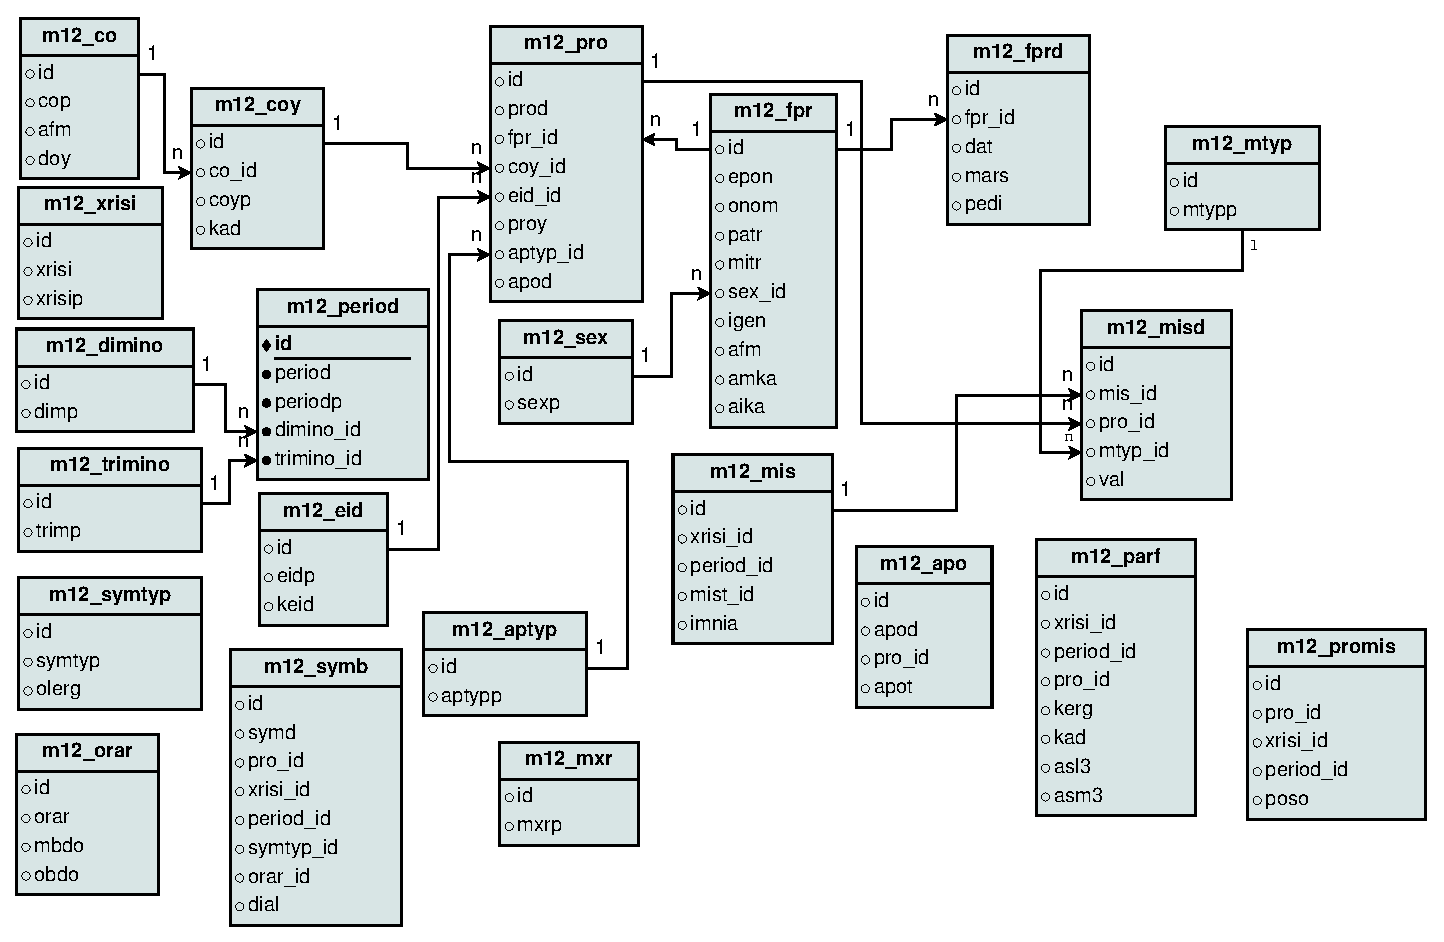
\includegraphics[width=150mm,height=80mm]{m13.eps}
\caption{Διάγραμμα ER της εφαρμογής}
\label{fig:diagrEr}
\end{figure}
Ακολουθεί λίστα με τους πίνακες της εφαρμογής (όνομα πίνακα και συνοπτική περιγραφή ).
\begin{enumerate}
\item apdp : Περίοδοι για την Αναλυτική περιοδική Δήλωση του ΙΚΑ . Ήταν κάθε τρίμηνο και τώρα έχει αλλάξει σε μηνιαία.
\item aptyp : Τύποι αποδοχών (Μισθός, ημερομίσθιο, ωρομίσθιο)
\item co : Στοιχεία εταιρείας. 'Ολα τα δεδομένα της επιχείρησης.
\item cotyp : Τύπος επιχείρησης ( 0.Εταιρεία, 1.Φυσικό πρόσωπο).
\item coy : Παράρτημα επιχείρησης .Υπάρχει τουλάχιστον ένα , το κεντρικό , που δημιουργείται αυτόματα κατά την δημιουργία νέας εταιρείας.
\item eid : Ειδικότητα εργασίας. Οι εγγραφές δημιουργούνται αυτόματα κατά την δημιουργία νέας εταιρείας ή νέου υποκαταστήματος με άλλο κωδικό δραστηριότητας από αυτόν του κεντρικού
\item fpr   : Στοιχεία Φυσικού Προσώπου  που παραμένουν αμετάβλητα.
\item fprd : Μεταβλητά στοιχεία Φυσικού προσώπου.
\item mis : Master πίνακας μισθοδοσίας
\item misd : Detail πίνακας μισθοδοσίας
\item mist : Tύπος μισθοδοσίας ( Τακτικές αποδοχές, Δώρο Πάσχα, Επίδομα Αδείας κλπ).
\item mtyp : Τύπος μισθολογικού δεδομένου ( Ημέρες εργασίας, Μισθός , ΙΚΑ , ποσοστό ΙΚΑ κλπ).
\item par : Master παρουσίας
\item pard : Detail παρουσίας
\item period : Περίοδος (Ιανουάριος, Φεβρουάριος κλπ).
\item pro : Πρόσληψη εργαζομένου.
\item ptyp : Τύπος παρουσίας.
\item sex : Φύλο (Άνδρας, Γυναίκα).
\item xrisi : Χρήση (2012, 2013 κλπ). 
\end{enumerate}
\subsection{SQL}
Όλες οι crud διαδικασίες γίνονται με sql. Υπάρχει ειδικό module που περιέχει τα sql strings και τους headers οργανωμένα για χρήση από τα υποσυστήματα της εφαρμογής.
\section{Gui - Φόρμες - Εκτυπώσεις}
\subsection{Gui}
Για να υπάρχει πλήρης ομογενοποίηση των gui στοιχείων στις φόρμες , χρησιμοποιούνται με subclassing τα παρακάτω :
\begin{enumerate}
\item DbLineEdit ( QLineEdit)
\item ButtonLineEdit (QLineEdit) . Το widget αυτό έχει τις καταστάσεις  εμφάνιση εγγραφής και εισαγωγή νέας εγγραφής. Κατά την εμφάνιση υπάρχουσας εγγραφής, δέχεται το id της εγγραφής και εμφανίζει την περιγραφή. Κατά την εισαγωγή νέας εγγραφής , ο χρήστης πατάει το κουμπάκι που υπάρχει δεξιά και εμφανίζει παράθυρο με λίστα επιλογών για να επιλέξει ο χρήστης. 
\item DbDateEdit (QDateEdit) για ημερομηνίες.  
\item WeekDays (QWidget). Custom widget για την επιλογή εργασίμων ημερών στη βδομάδα.
\item DbSpinBox (QSpinBox) για ακέραιες τιμές.
\item DbDoubleSpinBox(QDoubleSpinBox) για decimal τιμές.
\item DbComboBox (QComboBox). Δέχεται μια λίστα δύο διαστάσεων για εύρος τιμών.
\end{enumerate}
Όλα τα widgets έχουν τις μεθόδους setVal και getVal
\subsection{Φόρμες}
Η διαδικασία δημιουργίας φορμών είναι αυτοματοποιημένη (εκτός μερικών εξαιρέσεων :-) ) στις εξής κατηγορίες :
\begin{enumerate}
\item Φόρμα βασισμένη στο QTableWidget.
\item Master - Detail φόρμα.
\item TreeView φόρμα.
\item Σειριακή απλή φόρμα.
\end{enumerate}
Σε όλες τις φόρμες υπάρχει η δυνατότητα εκτύπωσης επακριβώς του περιεχομένου τους.
\section{Επικοινωνίες με άλλα συστήματα}
\section{Διαδικασίες Backup - Restore - Αναβάθμισης}
Όλα τα δεδομένα αποθηκεύονται σε αρχεία sqlite ,οπότε είναι πολύ εύκολη η διαδικασία του backup. Αυτό μπορεί να γίνει με δύο τρόπους :
\begin{enumerate}
\item Με απλή αντιγραφή του αρχείου.
\item Με δημιουργία αρχείου με sql δεδομένα.
\end{enumerate}
\section{Υποσυστήματα}
\subsection{Υπολογισμοί}
Για τον υπολογισμό μισθοδοσίας λαμβάνονται υπ'όψιν οι εξής παράμετροι:
\begin{enumerate}
\item Με την δημιουργία νέας εταιρείας , ζητούνται από το χρήστη τα βασικά δεδομένα που είναι ο κωδικός αριθμός δραστηριότητας για το κεντρικό, ο αριθμός μητρώου ΙΚΑ , ο κωδικός υποκαταστήματος του ΙΚΑ
\item Με τη δημιουργία νέας εταιρείας και με την επιλογή δραστηριότητας , έχουν ήδη εισαχθεί οι ειδικότητες που μπορεί να απασχολήσει η εταιρεία, όσον αφορά τα δεδομένα του ΙΚΑ. Όσον αφορά επικουρικά ταμεία χρειάζεται να γίνει ενημέρωση της ειδικότητας με τα στοιχεία αυτά.
\item Με τη δημιουργία νέου εργαζομένου , έχει γίνει εισαγωγή των βασικών του στοιχείων . Σε περίπτωση που προκύπτει εισαγωγή επικουρικού ταμείου , χρειάζεται να γίνουν απαραίτητες ενέργειες. Πάντως υπάρχει κάτι κοινό που επιδρά σε μεγάλο αριθμό επικουρικών ταμείων και αυτό είναι αν ο εργαζόμενος είναι ασφαλισμένος πριν από το 1983 ή μετά.
\item Υπάρχουν διάφοροι τύποι μισθοδοσίας : Μισθοδοσία περιόδου, ασθένειας, υπερωριών, κλπ. Για κάθε εργαζόμενο υπολογίζονται 15 μισθοδοσίες : 12 για τις περιόδους Ιανουάριο - Δεκέμβριο, 2 για δώρο Πάσχα και δώρο Χριστουγέννων και 1 για το επίδομα αδείας. Υπάρχουν ακόμα ειδικές όπως το επίδομα ισολογισμού, το bonus, οι δεδουλευμένες άδειες κλπ.
\item Υπάρχουν διάφοροι τύποι παρουσιών / απουσιών : Κανονικές εργάσιμες, σε κανονική άδεια, μέρες ασθένειας λιγότερες από 3 ή περισσότερες από 3, υπερεργασία, νυχτερινή προσαύξηση, υπερωρίες, κυριακές - αργίες, αδικαιολόγητη απουσία, δικαιολογημένη απουσία χωρίς αποδοχές κλπ
\end{enumerate}

Η διαδικασία γίνεται ως εξής :
\begin{enumerate} 

\item Επιλέγεται η περίοδος της μισθοδοσίας που μπορεί να λάβει τις Τιμές :
\begin{enumerate} 
\item Ιανουάριος - Δεκέμβριος 
\item Δώρο Πάσχα ή Δώρο Χριστουγέννων
\item Επίδομα Αδείας
\item Ειδικές περίοδοι όπως επίδομα ισολογισμού, bonus, δεδουλευμένες άδειες, αποζημίωση απόλυσης κλπ
\end{enumerate}
\item Για κάθε ενεργό εργαζόμενο:
\begin{enumerate} 
\item Γίνεται αυτόματη εισαγωγή των προεπιλεγμένων παρουσιών για την περίοδο.
\item Εφ'οσον πρόκειται για περίοδο πραγματικής εργασίας , γίνεται συμπλήρωση / διόρθωση των αυτόματα εισαχθέντων δεδομένων.
\end{enumerate}
\item Γίνεται οριστικοποίηση εισαγωγής δεδομένων παρουσιών για την περίοδο.
\item Μπορεί πλέον να γίνει ο υπολογiσμός της μισθοδοσίας. Μετά την ολοκλήρωση του υπολογισμού , γίνεται αποθήκευση των αποτελεσμάτων στην database.

\end{enumerate}

Στη συνέχεια γίνεται ο υπολογισμός και αποθήκευση των αποτελεσμάτων στη database.

 
\end{document}